\scanpage{258}
% letterhead
U N I V E R S I T E\hfill Montpellier, le 24 juin 1975\\
DES SCIENCES ET TECHNIQUES\\
\uline{DU LANGUEDOC}\\
AMC/MD

\uline{Diffusion} : Liste A\\
n° 4135

% printed form
AVIS DE SOUTENANCE D'UNE THESE DE DOCTORAT DE

\uline{SPECIALITE : CHIMIE}

Mention Chimie Organique Physique

\uline{Nom et prénom du candidat} : DALVERNY Gilbert

\uline{Titre de la thèse} : Synthèse et réactivité d'organomagnésiens perfluorés. Application à la préparation d'acides perfluorosulfoniques et carboxyliques.

\uline{Date, heure et lieu de soutenance prévus} : 10 juillet 1975 à 11 heures, salle de cours n° 9 - U.S.T.L.

\uline{Nom du Directeur de thèse} : Monsieur le Professeur A. COMMEYRAS

\uline{Désignation du laboratoire où la thèse est préparée} : Laboratoire de chimie organique

\uline{Analyse de l'ouvrage} : Des méthodes de synthèses, par voie chimique, d'acides perfluoroalcanesulfoniques $\mathrm{R_FSO_3H}$ et carboxyliques $\mathrm{R_FCO_2H}$ ont été mises au point ; elles font intervenir comme intermédiaires réactionnels, les organomagnésiens perfluorés saturés $\mathrm{R_FMgX}$ correspondants.

Des possibilités d'application de la réaction magnésienne au niveau de composés perfluorés insaturés ont été ensuite étudiées.

\uline{Durée approximative des recherches ayant abouti à la thèse} : 2 ans

\uline{Composition du jury proposé} : M. A. COMMEYRAS - Président\\
M. R. CORRIU\\
M. A. CAMBON\\
M. R. MARTIN

Le Secrétaire Général,\\
\figure{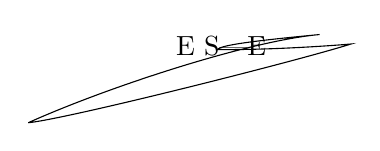
\begin{tikzpicture}[x=1cm,y=1cm]\draw (0,0) .. controls (1,.45) and (2.8,1.04) .. (3.7,1.12) .. controls (2.75,1.03) and (2.45,.98) .. (2.4,.93) .. controls (3.1,.92) and (4,.99) .. (4.1,1) .. controls (3.4,.78) and (.5,.05) .. (0,0);\node at (2.45,.97) {\handwritten{\unsure{E S|E}}};\end{tikzpicture}}
\uline{E. SIAU}
% archive sheet number: 257
